\documentclass{article}
\usepackage{tabularx}
\usepackage{graphicx}
\usepackage{dirtytalk}
\usepackage{pgfplotstable} 
\usepackage{pgfplots}
\usepackage{datatool}
\usepackage{siunitx}
\usepackage[hyphens]{url}
\usepackage{hyperref}
\usepackage{graphicx}
\usepackage{microtype}
\usepackage{float}
\usepackage[style=ieee]{biblatex}
\usepackage{listings}
\usepackage{xcolor}
\usepackage[normalem]{ulem}
\usepackage{dirtytalk}

\definecolor{mygreen}{rgb}{0,0.6,0}
\definecolor{mygray}{rgb}{0.5,0.5,0.5}
\definecolor{mymauve}{rgb}{0.58,0,0.82}

\lstset{
    language=Java,                % Set language to Java
    basicstyle=\ttfamily\footnotesize, % Set font style and size
    keywordstyle=\color{blue},    % Set color for keywords
    stringstyle=\color{mymauve},  % Set color for strings
    commentstyle=\color{mygreen}, % Set color for comments
    numbers=left,                 % Line numbers on the left
    numberstyle=\tiny\color{mygray}, % Style for line numbers
    stepnumber=1,                 % Line number step size
    numbersep=10pt,               % Line number separation
    backgroundcolor=\color{white},% Background color
    showspaces=false,             % Do not show spaces
    showstringspaces=false,       % Do not underline spaces in strings
    showtabs=false,               % Do not show tabs
    frame=single,                 % Draw a frame around the code
    tabsize=4,                    % Set tab size
    captionpos=b,                 % Caption position (bottom)
    breaklines=true,              % Allow line breaking
    breakatwhitespace=false,      % Line breaks only at whitespace
    title=\lstname                % Show the filename of the code
}

\lstdefinestyle{bash}{
    language=bash,                % Set language to Bash
    basicstyle=\ttfamily\footnotesize, % Set font style and size
    keywordstyle=\color{blue},    % Set color for keywords
    stringstyle=\color{mymauve},  % Set color for strings
    commentstyle=\color{mygreen}, % Set color for comments
    numbers=left,                 % Line numbers on the left
    numberstyle=\tiny\color{mygray}, % Style for line numbers
    stepnumber=1,                 % Line number step size
    numbersep=10pt,               % Line number separation
    backgroundcolor=\color{white},% Background color
    showspaces=false,             % Do not show spaces
    showstringspaces=false,       % Do not underline spaces in strings
    showtabs=false,               % Do not show tabs
    frame=single,                 % Draw a frame around the code
    tabsize=4,                    % Set tab size
    captionpos=b,                 % Caption position (bottom)
    breaklines=true,              % Allow line breaking
    breakatwhitespace=false,      % Line breaks only at whitespace
    title=\lstname                % Show the filename of the code
}

\addbibresource{main.bib}

\hypersetup{
    colorlinks=true,
    linkcolor=blue,
    filecolor=blue,      
    urlcolor=blue,
    citecolor=blue,
}

\pgfplotsset{compat=1.18}

\title{\textbf{Lab 3 - Linearizability of Lock-free Skiplists\\Parallel and Distributed Computing\\DD2443 - Pardis24}}
\author{Names:\\Casper Kristiansson\\Nicole Wijkman\\\\Group 14}
\date{\today}

\begin{document}

\setlength\parindent{0pt}
\setlength{\parskip}{\bigskipamount}

\maketitle

\newpage
\section{Measuring Execution Time}

\subsection{Measurement program}

\subsubsection{Explanation}
We used the provided program to test the execution time of the LockFreeSkipList with 1, 2, 4, and 8 threads. The operations were distributed as 10\% add, 10\% remove, and 80\% contains (1:1:8), and values were sampled using both normal and uniform distributions. Each thread performed 100,000 operations. The program was run with 5 warmup rounds and 10 measurement rounds for final statistics.

\subsubsection{Results}



\textbf{Table 1: Execution Time for Uniform Distribution (1:1:8)}

\begin{table}[H]
    \centering
    \begin{tabular}{|c|c|c|}
    \hline
    \textbf{Threads} & \textbf{Warmup Time (ns)} & \textbf{Measurement Time (ns)} \\ \hline
    1 & 55,096,875 & 35,600,292 \\ 
    2 & 109,675,583 & 44,935,459 \\
    4 & 363,937,458 & 56,631,625 \\
    8 & 256,145,416 & 164,120,625 \\
    \hline
    \end{tabular}
    \caption{Execution Times for Uniform Distribution (1:1:8)}
\end{table}

\textbf{Table 2: Execution Time for Normal Distribution (1:1:8)}

\begin{table}[H]
    \centering
    \begin{tabular}{|c|c|c|}
    \hline
    \textbf{Threads} & \textbf{Warmup Time (ns)} & \textbf{Measurement Time (ns)} \\ \hline
    1 & 57,497,208 & 38,499,292 \\ 
    2 & 123,921,375 & 53,888,125 \\
    4 & 161,396,209 & 85,163,125 \\
    8 & 275,319,833 & 144,458,709 \\
    \hline
    \end{tabular}
    \caption{Execution Times for Normal Distribution (1:1:8)}
\end{table}

\subsubsection{Discussion}
The results show that as the number of threads increases, the execution time initially decreases but then increases again, especially with 8 threads. This suggests that the overhead of managing threads outweighs the benefits of parallelism beyond 4 threads in this case.


\newpage
\subsection{Dardel Experiments}

\subsubsection{Explanation}
The Dardel experiments used thread counts of 1, 2, 4, 8, 16, 32, 64, and 96 to test the skiplist implementation. Two types of distributions were tested: uniform and normal. Two operation mixtures were evaluated:
\begin{itemize}
    \item A.1: 10\% add, 10\% remove, and 80\% contains
    \item A.2: 50\% add and 50\% remove
\end{itemize}
These setups simulated varying workloads, with a mix of read-heavy and balanced operations.

\subsubsection{Results and Plots}
The plots show the average execution time (in nanoseconds) for each distribution and operation mixture, with the x-axis representing the number of threads and the y-axis showing execution time.

\begin{figure}[H]
    \centering
    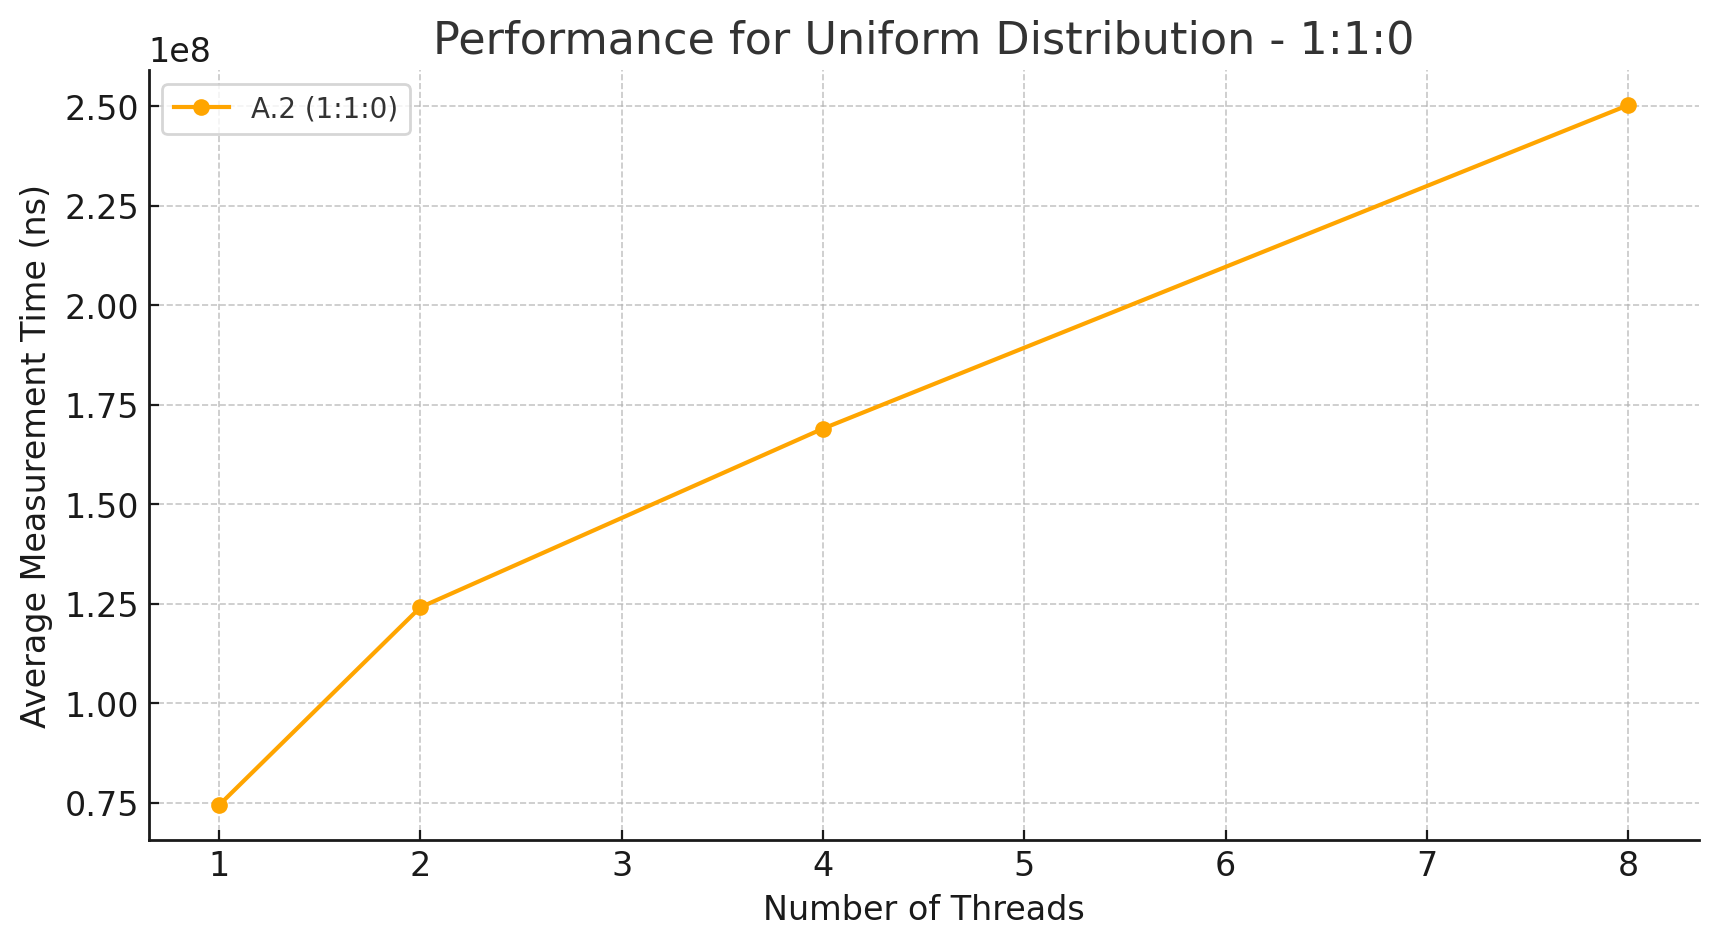
\includegraphics[width=\textwidth]{LaTex/images/Lab 3 1.2.1.png}
    \caption{Performance for Uniform Distribution - 1:1:0}
    \label{fig:enter-label}
\end{figure}

\begin{figure}[H]
    \centering
    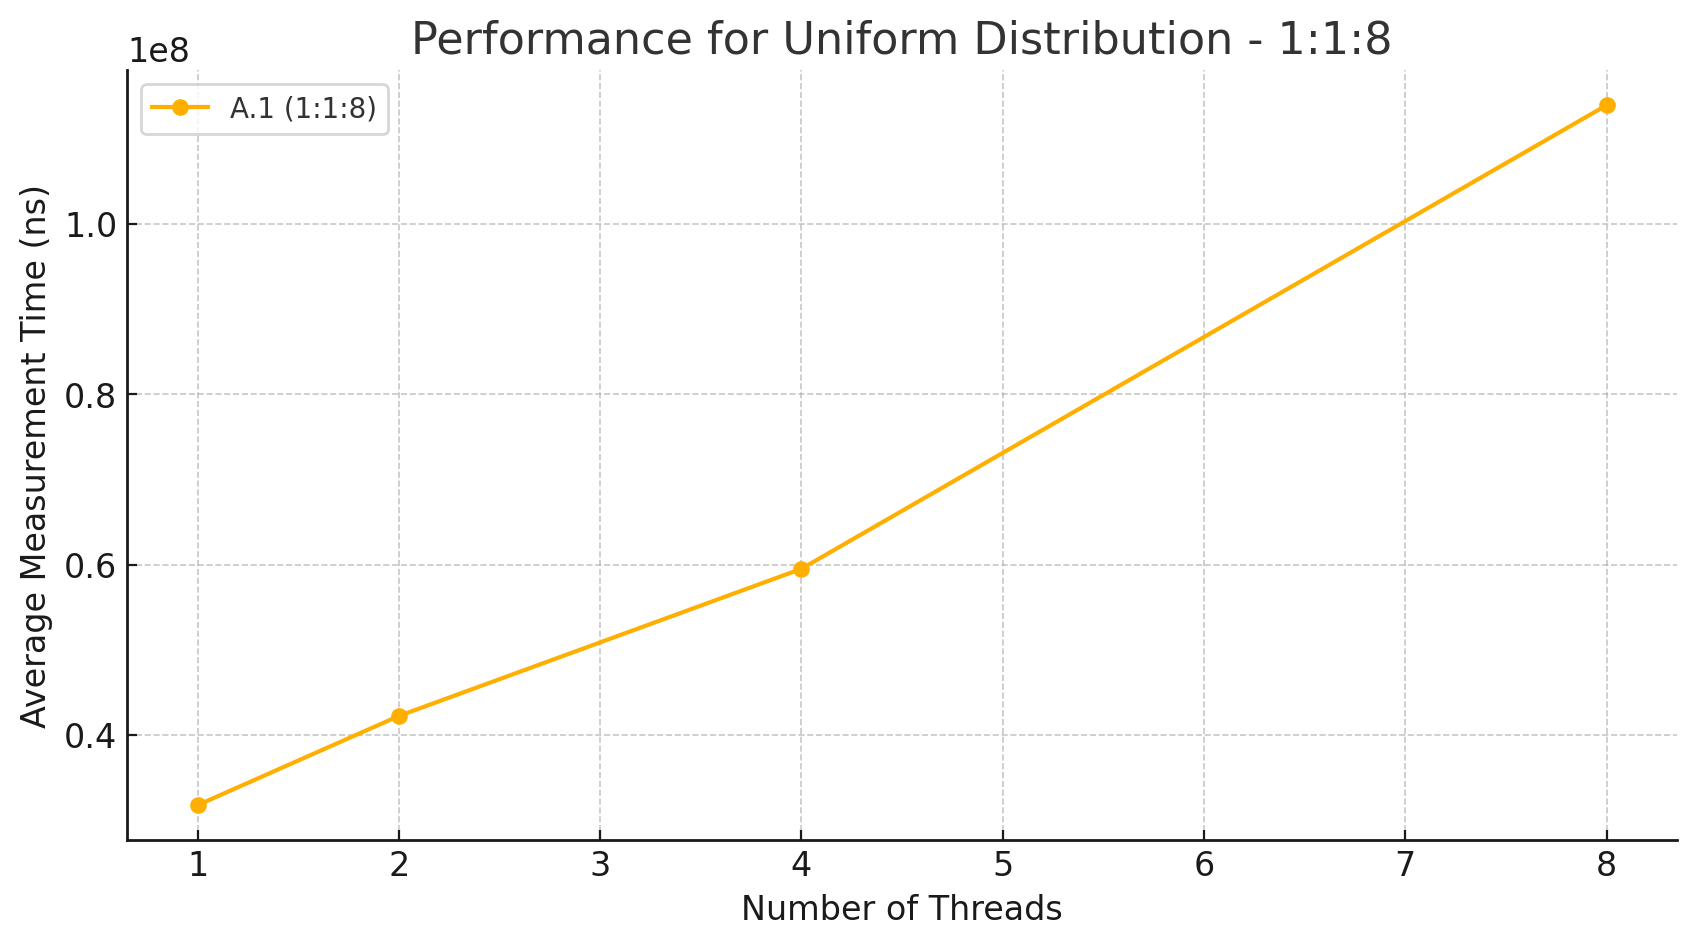
\includegraphics[width=\textwidth]{LaTex/images/Lab 3 1.2.2.png}
    \caption{Performance for Uniform Distribution - 1:1:8}
    \label{fig:enter-label}
\end{figure}

\subsubsection{Discussion}
The results show that as the number of threads increases, execution time also increases. In A.1 (1:1:8), the read-heavy workload initially scales well but suffers from increased contention with more threads. In A.2 (1:1:0), the balanced operation mix results in higher execution times, especially due to the overhead of frequent insertions and deletions. The sharp rise in execution time beyond 4 threads suggests contention from shared resources is the main bottleneck.


\newpage
\section{Identifying and Validating Linearization Points}

\subsection{Identify Linearization Points}

\subsubsection{Explanation}
In the \texttt{LockFreeSkipList}, linearization points are the moments when operations appear to take effect atomically. These points ensure correctness in a concurrent environment.

For the \texttt{add()} method, the linearization point occurs when the \texttt{compareAndSet()} succeeds on the bottom-level reference, linking the new node into the list. If the node is already present, the linearization point is during the \texttt{find()} operation that detects the node’s presence.

In the \texttt{remove()} method, the linearization point of \texttt{remove()} occurs when a successful \texttt{compareAndSet()} marks the bottom-level node for removal (line 96 in the source code). For unsuccessful removals, the \texttt{find()} method is not the linearization point itself; rather, it helps in identifying the linearization point by determining whether a node has been logically removed (marked) in combination with other operations like \texttt{compareAndSet()}.

The \texttt{contains()} method’s linearization point happens when it checks the bottom-level list and observes whether the target node is unmarked. Success occurs when the target key is found, and failure when the key is missing.


\subsubsection{Discussion}
The linearization points for \texttt{add()}, \texttt{remove()}, and \texttt{contains()} are all based on atomic \texttt{compareAndSet()} operations, ensuring consistency across threads. In \texttt{add()} and \texttt{remove()}, it’s crucial to manage concurrent attempts to modify the same node, while \texttt{contains()} ensures it reflects the correct presence of the node. By placing linearization points at key \texttt{compareAndSet()} operations, we maintain the appearance of atomicity, which is vital for ensuring correct and efficient concurrent behavior.



\newpage
\subsection{Developing a Validation Method}

\subsubsection{Explanation}
The \texttt{LogEntry} class was designed to capture the linearization points by recording the method name (for example: \texttt{add()}, \texttt{remove()}, or \texttt{contains()}), the arguments (the hash code of the element), the return value (e.g., success or failure), and the exact timestamp using \texttt{System.nanoTime()}. For validation, the \texttt{Log.validate} method replays the log entries on a \texttt{HashSet} and compares the results. If the \texttt{add()} method returns true in the log but the \texttt{HashSet} shows it as false, this counts as a discrepancy. The number of discrepancies indicates the consistency of the log.

\subsubsection{Discussion}
The validation method worked effectively for capturing the linearization points for the \texttt{add()} and \texttt{remove()} operations, resulting in a low discrepancy count. The challenge was ensuring that the \texttt{contains()} method properly captures linearization points, as this operation only checks for the existence of an element and does not modify the skiplist, making it harder to validate with the same accuracy as \texttt{add()} and \texttt{remove()}. However, the overall log validation showed consistent and reliable behavior.

\newpage
\subsection{Locked Time Sampling}

\subsubsection{Explanation}
The locked time sampling method was implemented by acquiring a \texttt{ReentrantLock} around the linearization point and the time sampling call. The lock ensures that no other thread can interleave between the linearization point and the time sampling, providing an accurate measurement. In the \texttt{remove()} method, after a successful \texttt{compareAndSet()}, the timestamp is captured using \texttt{System.nanoTime()}, ensuring atomicity between the linearization point and the time sampling. This pattern is also followed in the \texttt{add()} and \texttt{contains()} methods, ensuring consistent and accurate time capture for each operation.

\subsubsection{Results and Plots}

The following plots show the performance of the locked time sampling method in different operation mixtures. The x-axis represents the number of threads, and the y-axis represents the measurement time in nanoseconds.

\begin{figure}[H]
    \centering
    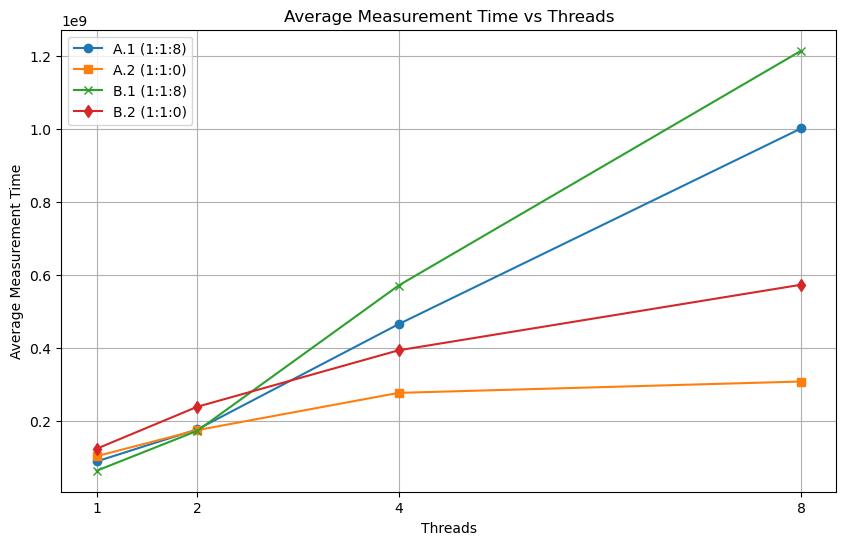
\includegraphics[width=\textwidth]{LaTex/images/Lab 3 2.3.2.1.png}
    \caption{Measurement Time vs Threads (A.1)}
    \label{fig:enter-label}
\end{figure}

\begin{figure}[H]
    \centering
    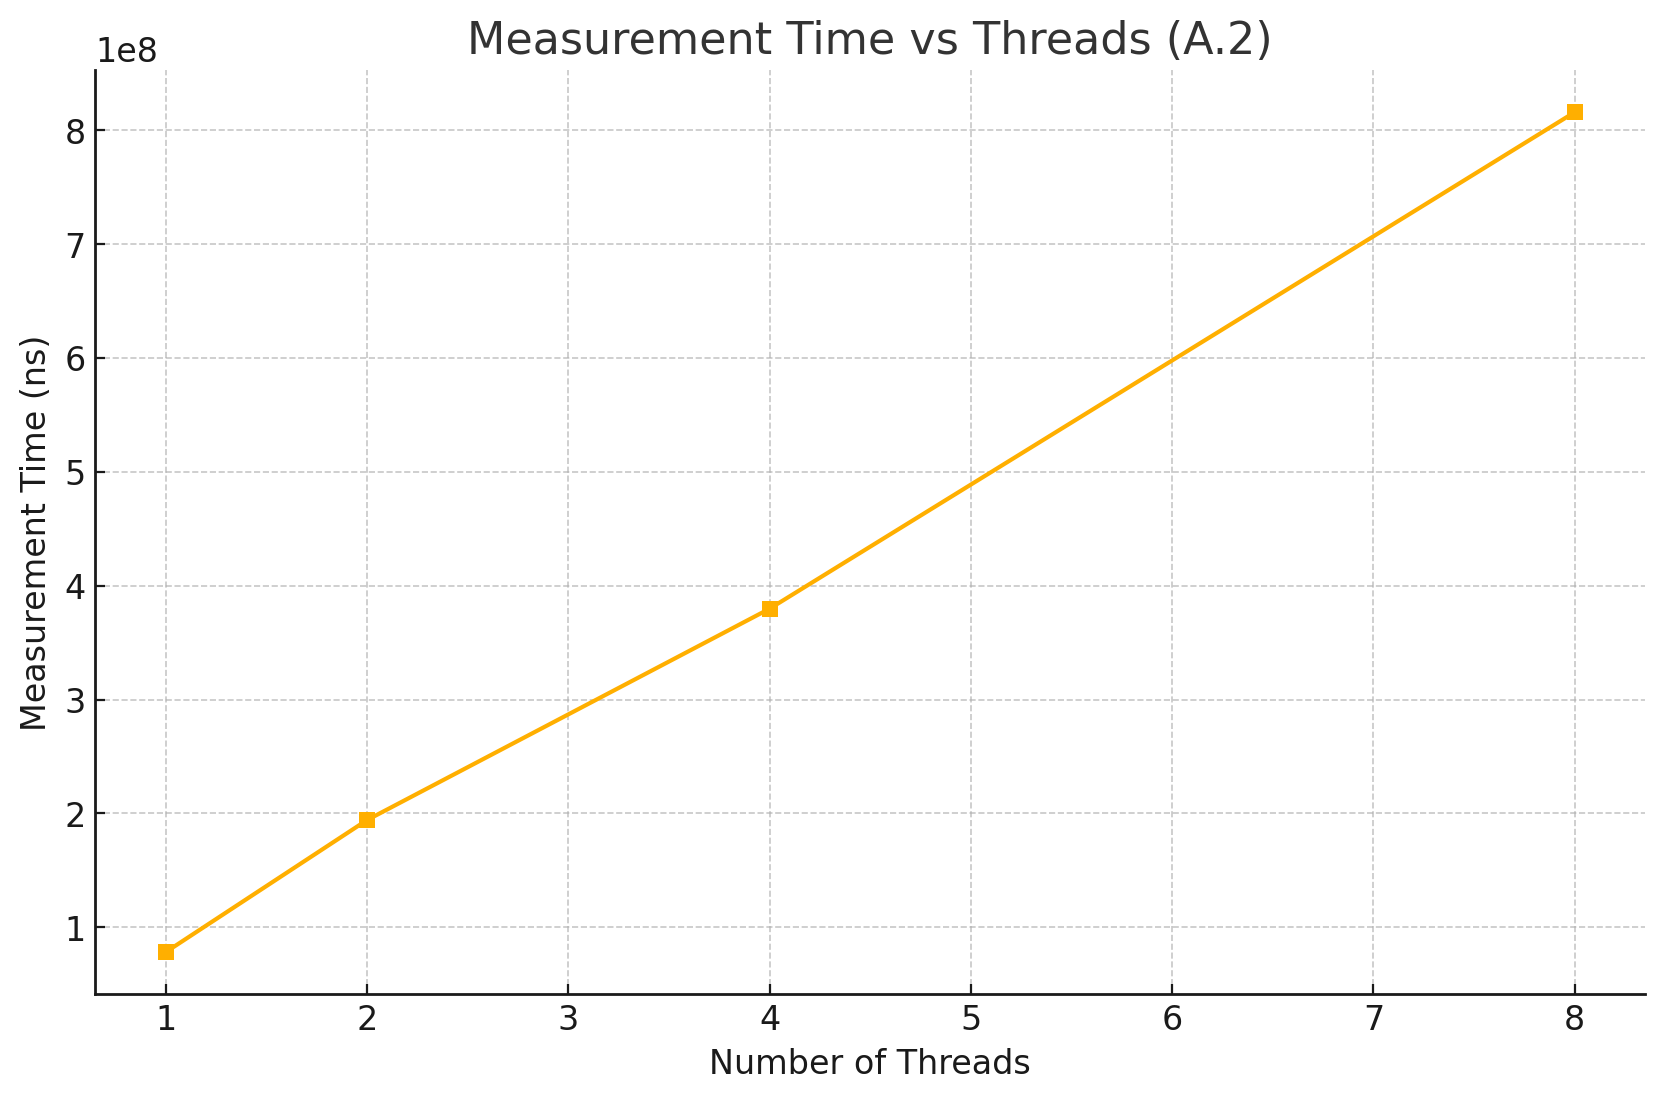
\includegraphics[width=\textwidth]{LaTex/images/Lab 3 2.3.2.2.png}
    \caption{Measurement Time vs Threads (A.2)}
    \label{fig:enter-label}
\end{figure}

\subsubsection{Discussion}
The performance of the locked time sampling method was satisfactory, though it introduced some latency due to the use of locks. When compared to the local measurement experiments, the locked implementation had a small lag but produced more accurate results. The discrepancies were minimal, as the locking mechanism ensured that the time sampling and linearization points remained synchronized.


\newpage
\subsection{Lock-free Time Sampling with Local Log}

\subsubsection{Explanation}
In the lock-free time sampling method, each thread maintains its own local log, storing time samples and log entries without using a global lock. Each thread independently logs its operations, and after the experiment concludes, the local logs are merged into a global log, which is sorted by timestamp and validated. The absence of global synchronization reduces overhead but introduces a risk of discrepancies, as the interval between time sampling and the linearization point is not protected.

\subsubsection{Results and Plots}

The following plots show the performance of the lock-free time sampling method with local logs in different operation mixtures. The x-axis represents the number of threads, and the y-axis represents the measurement time in nanoseconds.

\begin{figure}[H]
    \centering
    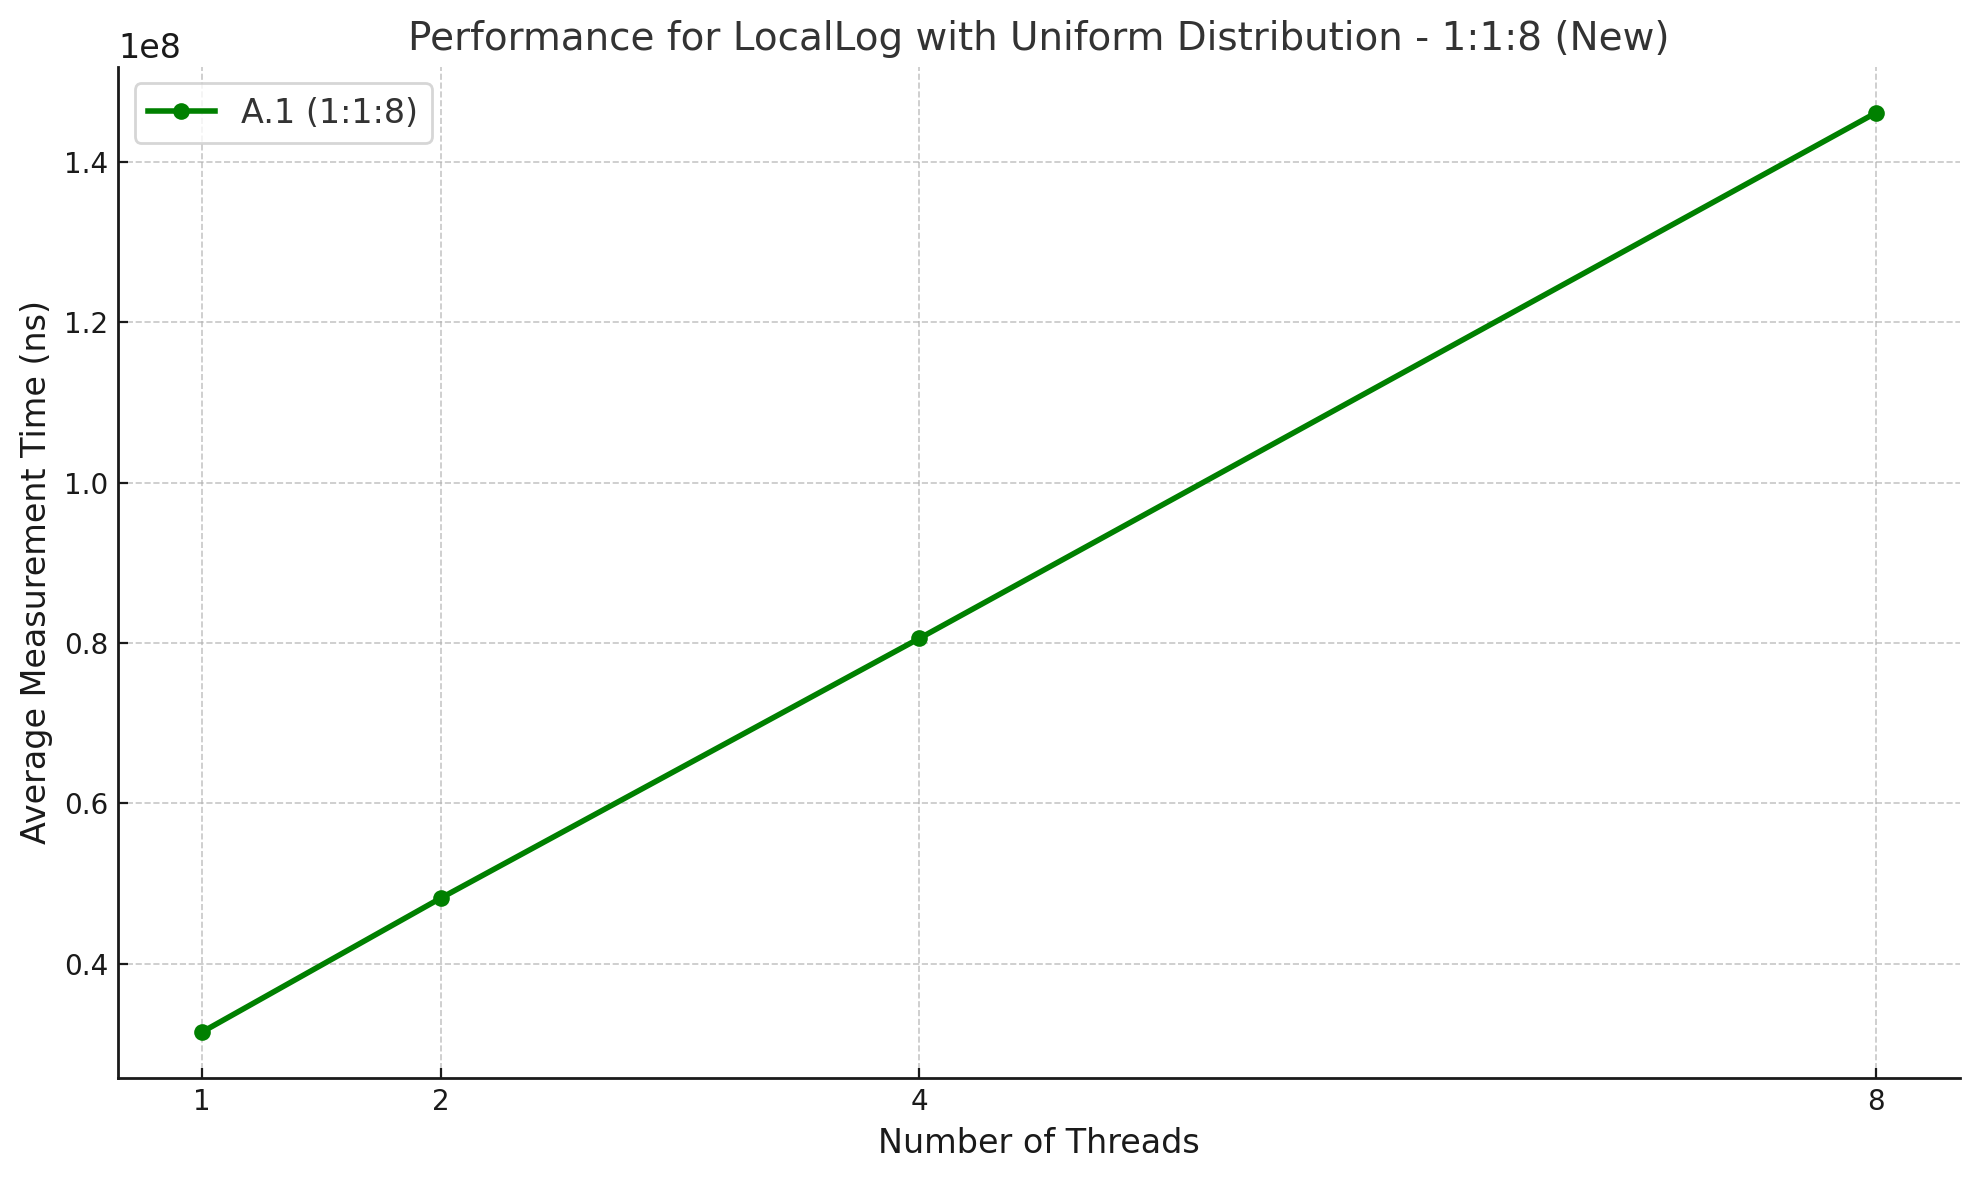
\includegraphics[width=\textwidth]{LaTex/images/Lab 3 2.4.2.1.png}
    \caption{Performance for LocalLog with Uniform Distribution - 1:1:8}
    \label{fig:performance_a1}
\end{figure}

\begin{figure}[H]
    \centering
    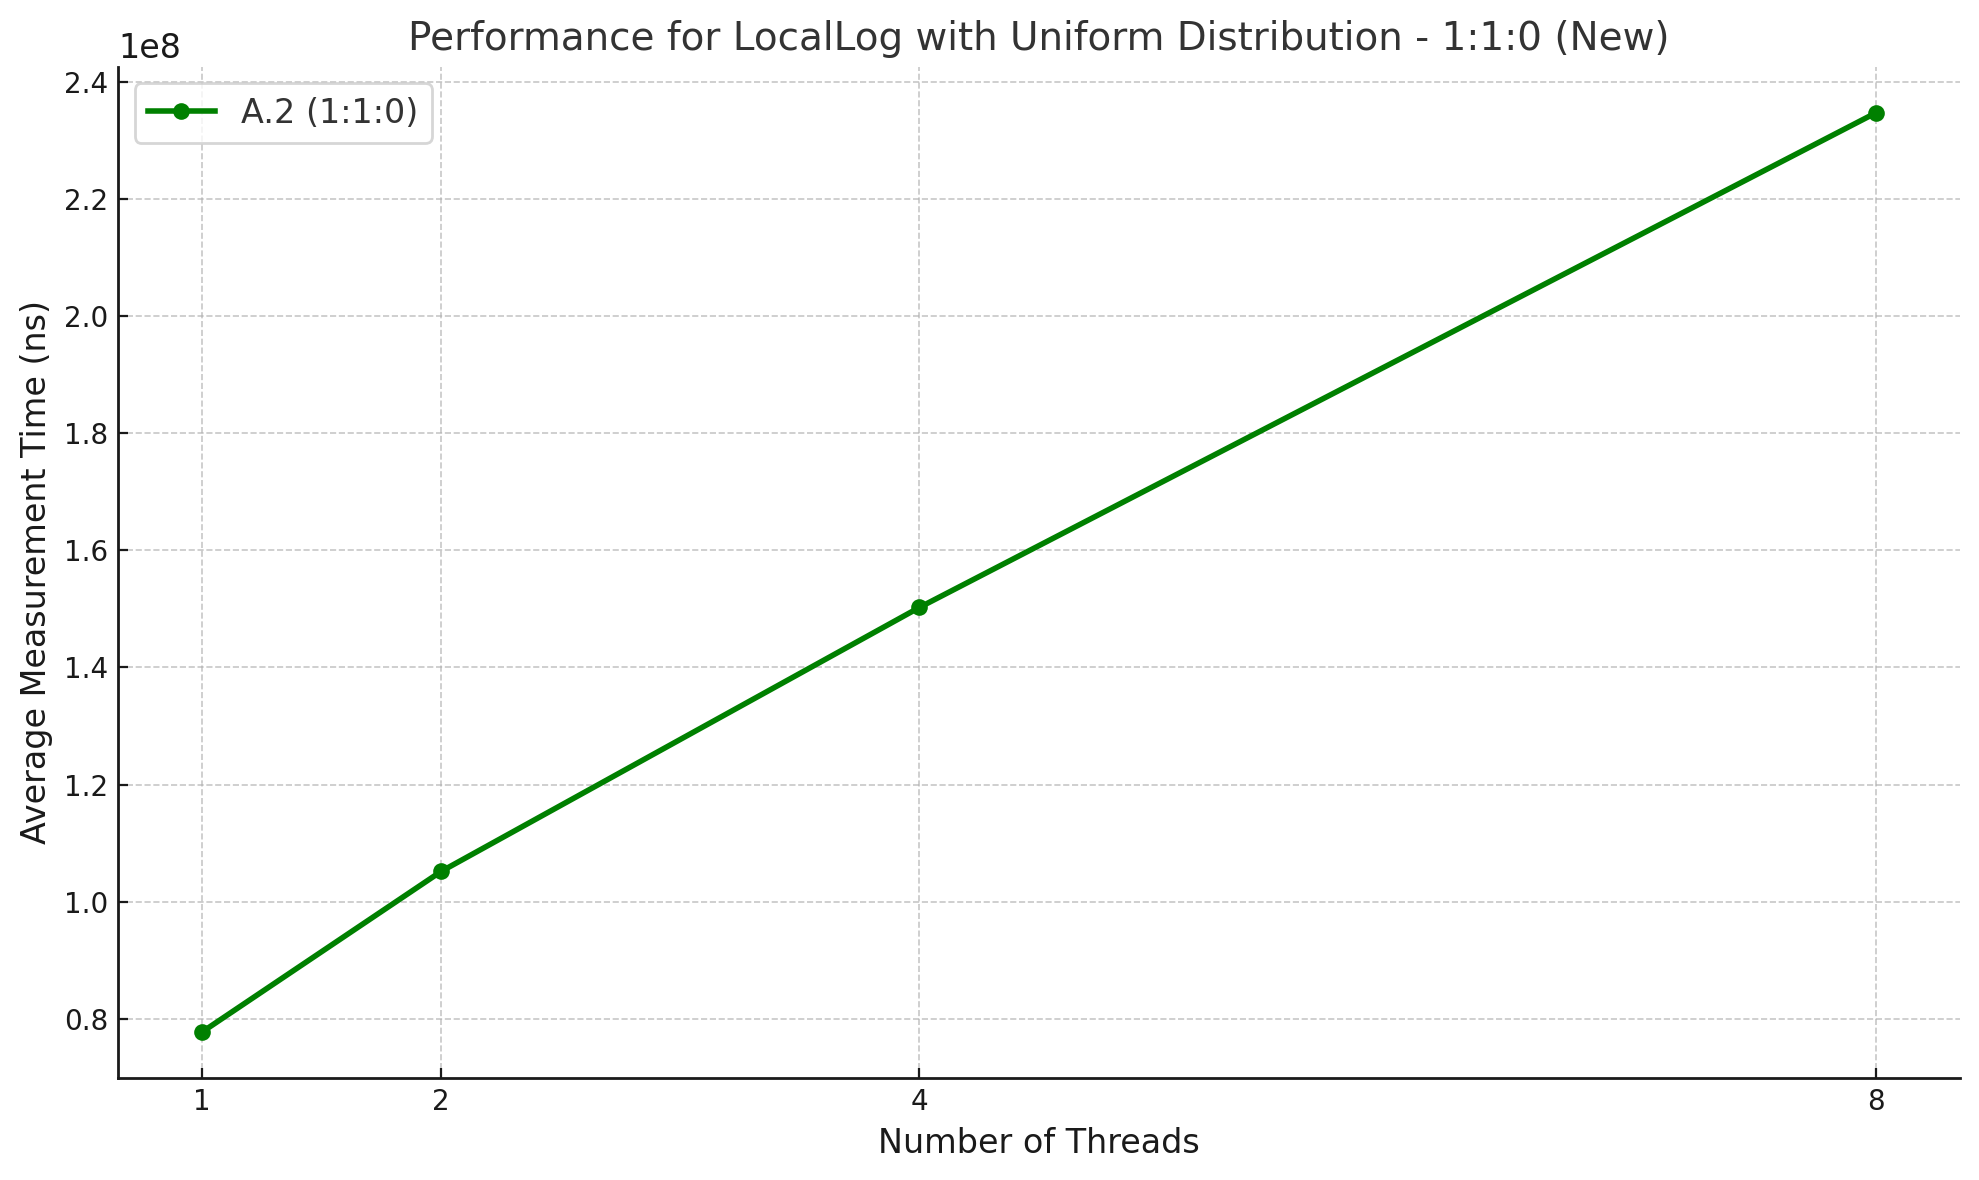
\includegraphics[width=\textwidth]{LaTex/images/Lab 3 2.4.2.2.png}
    \caption{Performance for LocalLog with Uniform Distribution - 1:1:0}
    \label{fig:performance_a2}
\end{figure}


\subsubsection{Discussion}
The lock-free local logging approach significantly reduces overhead by eliminating global locking, which improves performance, especially with lower thread counts. As shown in the table, when the number of threads was 1, 2, or 4, the discrepancy count remained at zero. This is because, with fewer threads, the likelihood of interleaving between time sampling and the linearization point is minimal, and the system can log entries consistently.

However, as the number of threads increased to 8, discrepancies began to appear. The increased concurrency led to overlapping execution and the absence of global synchronization introduced slight mismatches between time sampling and the actual linearization point. Despite this, the discrepancy count remained low, indicating acceptable accuracy for this workload.

The method effectively scales with minimal discrepancy at lower thread counts, making it a suitable choice for workloads with fewer threads or less contention. The zero-discrepancy results for lower thread counts highlight the method's efficiency in those conditions.


\newpage
\subsection{Lock-free Time Sampling with Global Log}

\subsubsection{Explanation}
The global lock-free time sampling method was implemented using a concurrent lock-free queue from \texttt{java.util.concurrent}. Each thread directly writes to the global log using non-blocking operations, minimizing synchronization overhead. Log entries are stored globally, and after all threads complete their operations, the entries are sorted and validated similarly to the local log approach.

\subsubsection{Results and Plots}

The following plots show the performance of the global lock-free time sampling method under two different operation mixtures. The x-axis represents the number of threads, and the y-axis represents the measurement time in nanoseconds.

\begin{figure}[H]
    \centering
    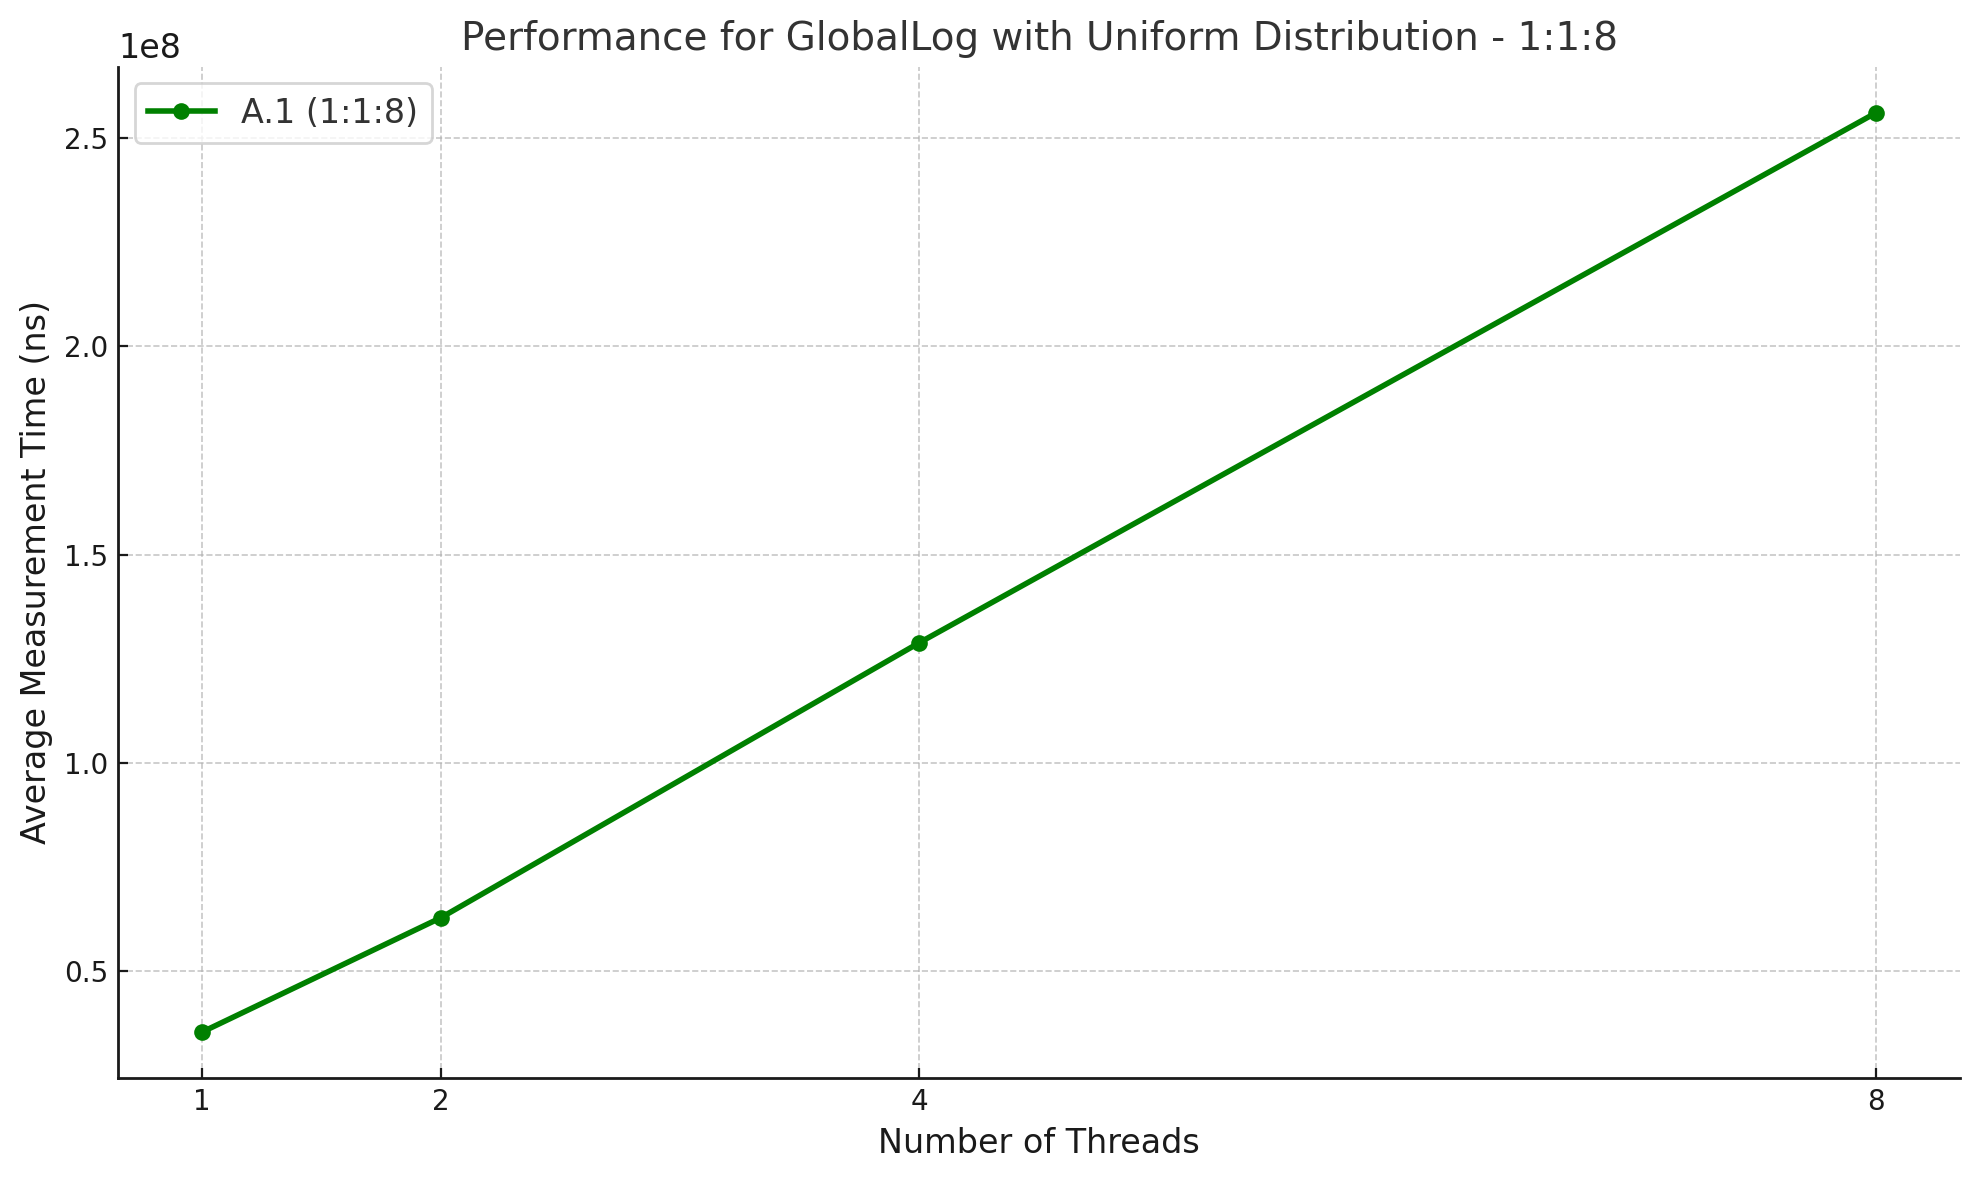
\includegraphics[width=\textwidth]{LaTex/images/Lab 3 2.5.2.1.png}
    \caption{Measurement Time vs Threads (A.1: 1:1:8)}
    \label{fig:global-log-1-1-8}
\end{figure}

\begin{figure}[H]
    \centering
    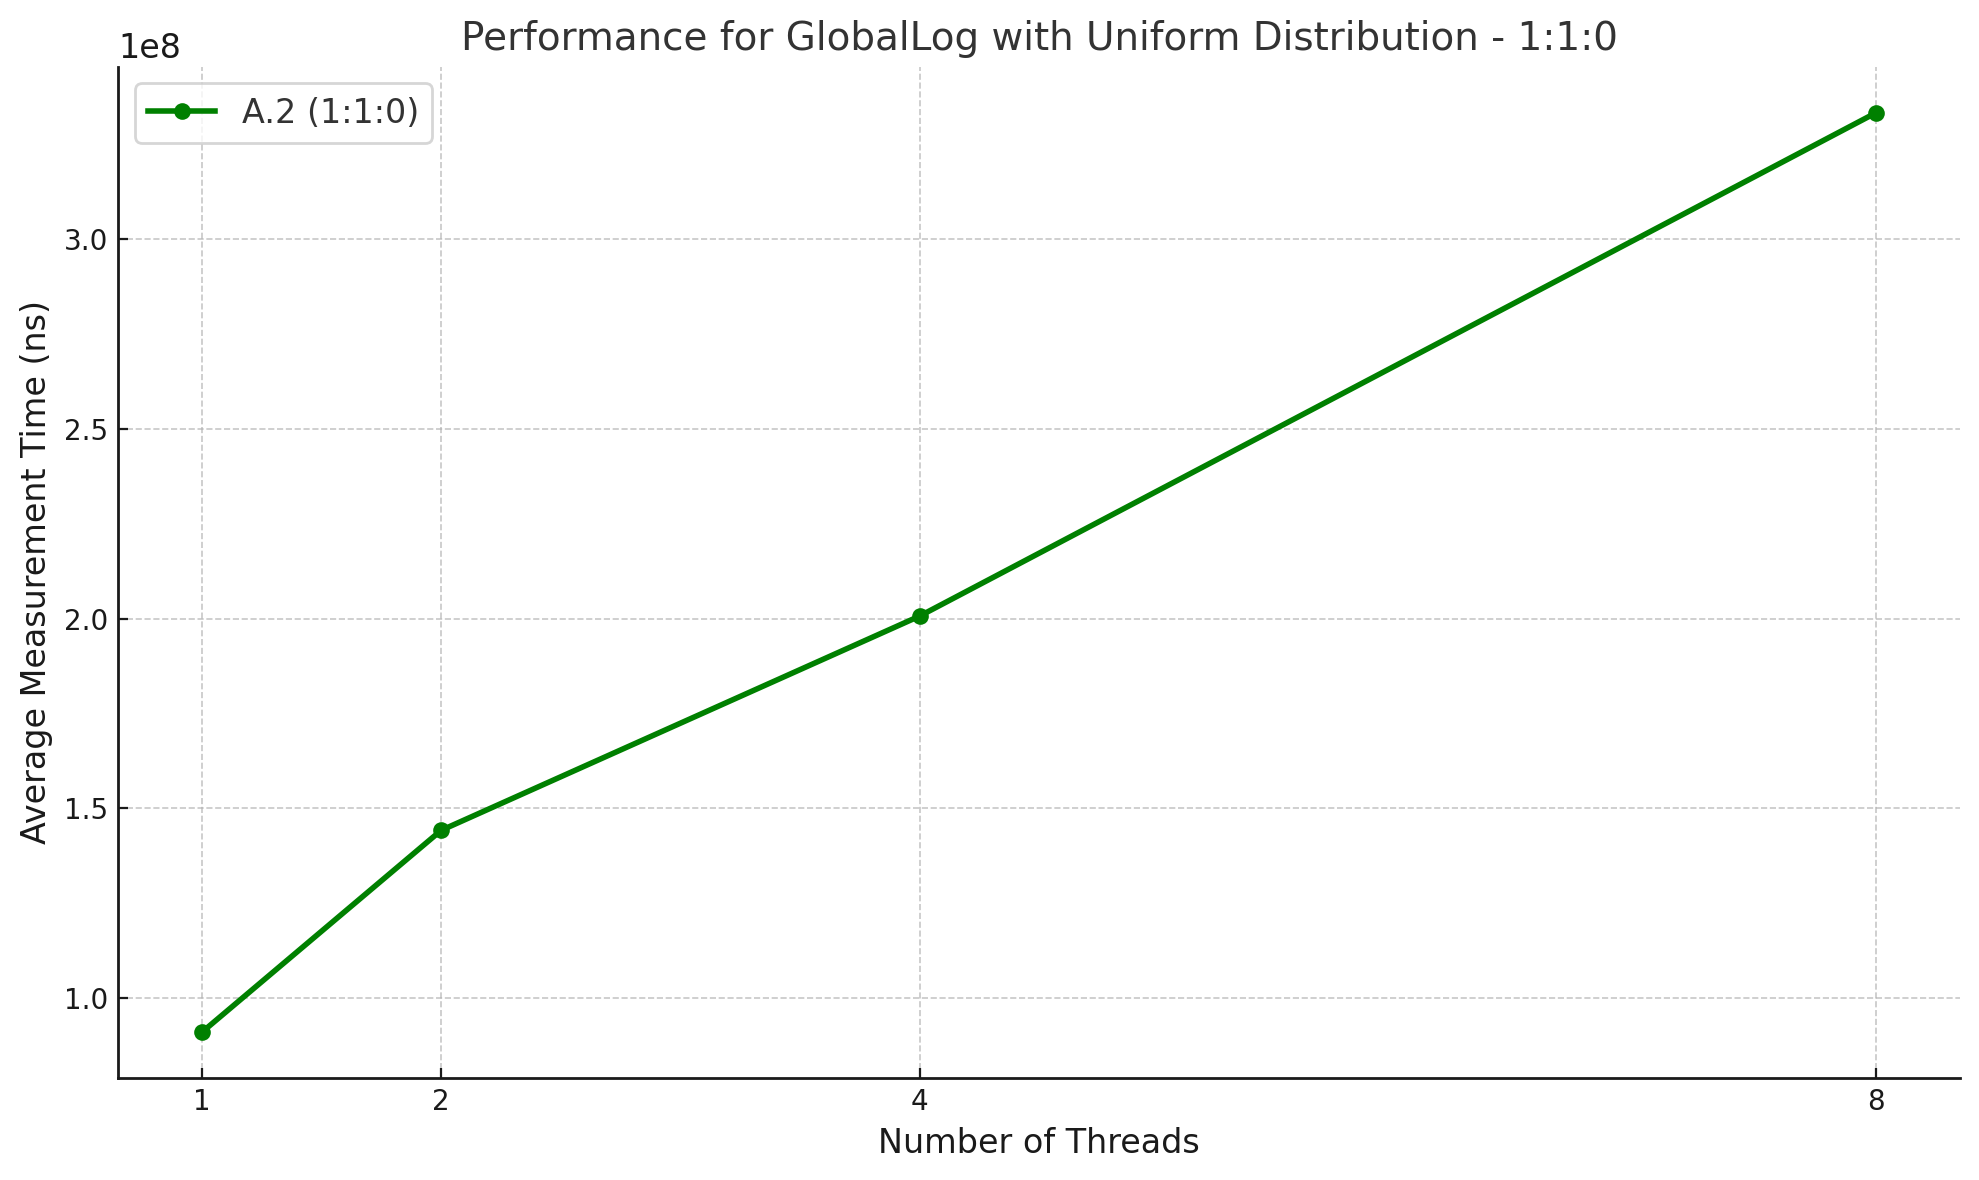
\includegraphics[width=\textwidth]{LaTex/images/Lab 3 2.5.2.2.png}
    \caption{Measurement Time vs Threads (A.2: 1:1:0)}
    \label{fig:global-log-1-1-0}
\end{figure}


\subsubsection{Discussion}
The global log time sampling method provided the best performance when compared to both local log and locked time sampling methods. By avoiding any global synchronization, this approach was able to handle higher thread counts with minimal performance degradation. The global log also scales well across increasing thread counts, as shown by the linear increase in measurement time in the plots.

However, this method introduced some minor discrepancies when the thread count increased to 8, as seen in the data. These discrepancies are not due to inaccuracies in \texttt{System.nanoTime()} but rather the lack of synchronization between time sampling and the linearization point. The non-blocking nature of the global log allows for slight interleaving of log entries, which introduces minor inconsistencies in the recorded linearization points.

Overall, despite the minor discrepancies at higher thread counts, the global log method proved to be highly scalable and efficient, making it a suitable choice for high-concurrency workloads where minimizing synchronization overhead is crucial.



\newpage
\subsection{Dardel Experiments for Log Accuracy}

\subsubsection{Setup and Results}
%Provide an overview of the experiments run on Dardel using the sampling methods from the previous sections. Include a plot of execution time and log accuracy.

\subsubsection{Discussion}
%Discuss the performance and accuracy results from the Dardel experiments. Compare the different sampling methods (locked, local log, global log) and explain which approach provided the best trade-off between performance and accuracy.

\newpage
\printbibliography

\end{document}
